%  Copyright 2020-2026 Robert Bosch GmbH
%
%  Licensed under the Apache License, Version 2.0 (the "License");
%  you may not use this file except in compliance with the License.
%  You may obtain a copy of the License at
%
%      http://www.apache.org/licenses/LICENSE-2.0
%
%  Unless required by applicable law or agreed to in writing, software
%  distributed under the License is distributed on an "AS IS" BASIS,
%  WITHOUT WARRANTIES OR CONDITIONS OF ANY KIND, either express or implied.
%  See the License for the specific language governing permissions and
%  limitations under the License.
\chapter{Roo Code Extension}

\section{Introduction}
Roo Code is an autonomous AI software engineer that operates directly within
the VSCodium.
Unlike standard AI assistants, Roo Code can interact with your file system,
execute terminal commands, and use a browser to provide a seamless,
agentic development experience.

\section{Installation}
Roo Code Extension is pre-installed in the \textbf{Robot Framework AIO} package.
To verify the installation:

\begin{itemize}
   \item Open \textbf{VSCodium For RobotFramework}.
   \item Navigate to the \textbf{Extensions} view (\texttt{Ctrl+Shift+X}).
   \item Search for \textbf{"Roo Code"}.
   \item Ensure the extension is enabled and
         the \textbf{"Roo Code"} icon should appear in the Activity Bar.
\end{itemize}
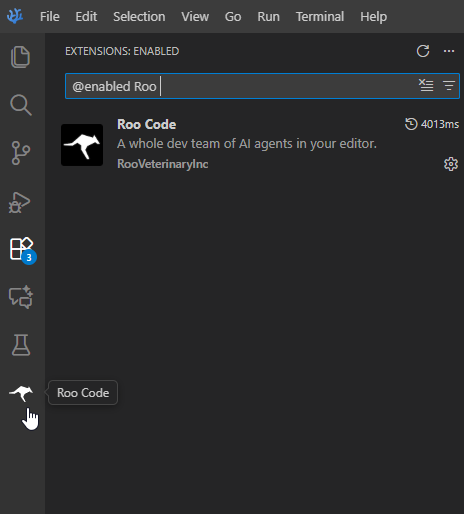
\includegraphics{./include/graphics/roocode/RooCodeExtension.png}

\section{Key Features}
Roo Code enhances the development experience in
\textbf{VSCodium For RobotFramework} with several "agentic" capabilities:
\begin{itemize}
   \item \textbf{Autonomous Coding:}
      Reads, writes, and creates files based on natural language.
   \item \textbf{Terminal Control:}
      Executes shell commands (e.g., running Robot Framework tests,
      installing pip packages) and self-fixes based on output.
   \item \textbf{Self-Healing Tests:}
      Automatically analyzes test failures and refactors code until tests pass.
   \item \textbf{Browser Integration:}
      Launches a headless browser to inspect UIs or gather documentation.
   \item \textbf{MCP Support:}
      Connects to external tools (Google Drive, GitHub, Slack) via the
      Model Context Protocol - MCP.
\end{itemize}

\section{Configuration}
Before using Roo Code, you must configure an AI Language Model.
You can choose between AI Prvoiders models, local models (via Ollama) or
GitHub Copilot.

Now, get started by selecting your preferred model provider as shown below:

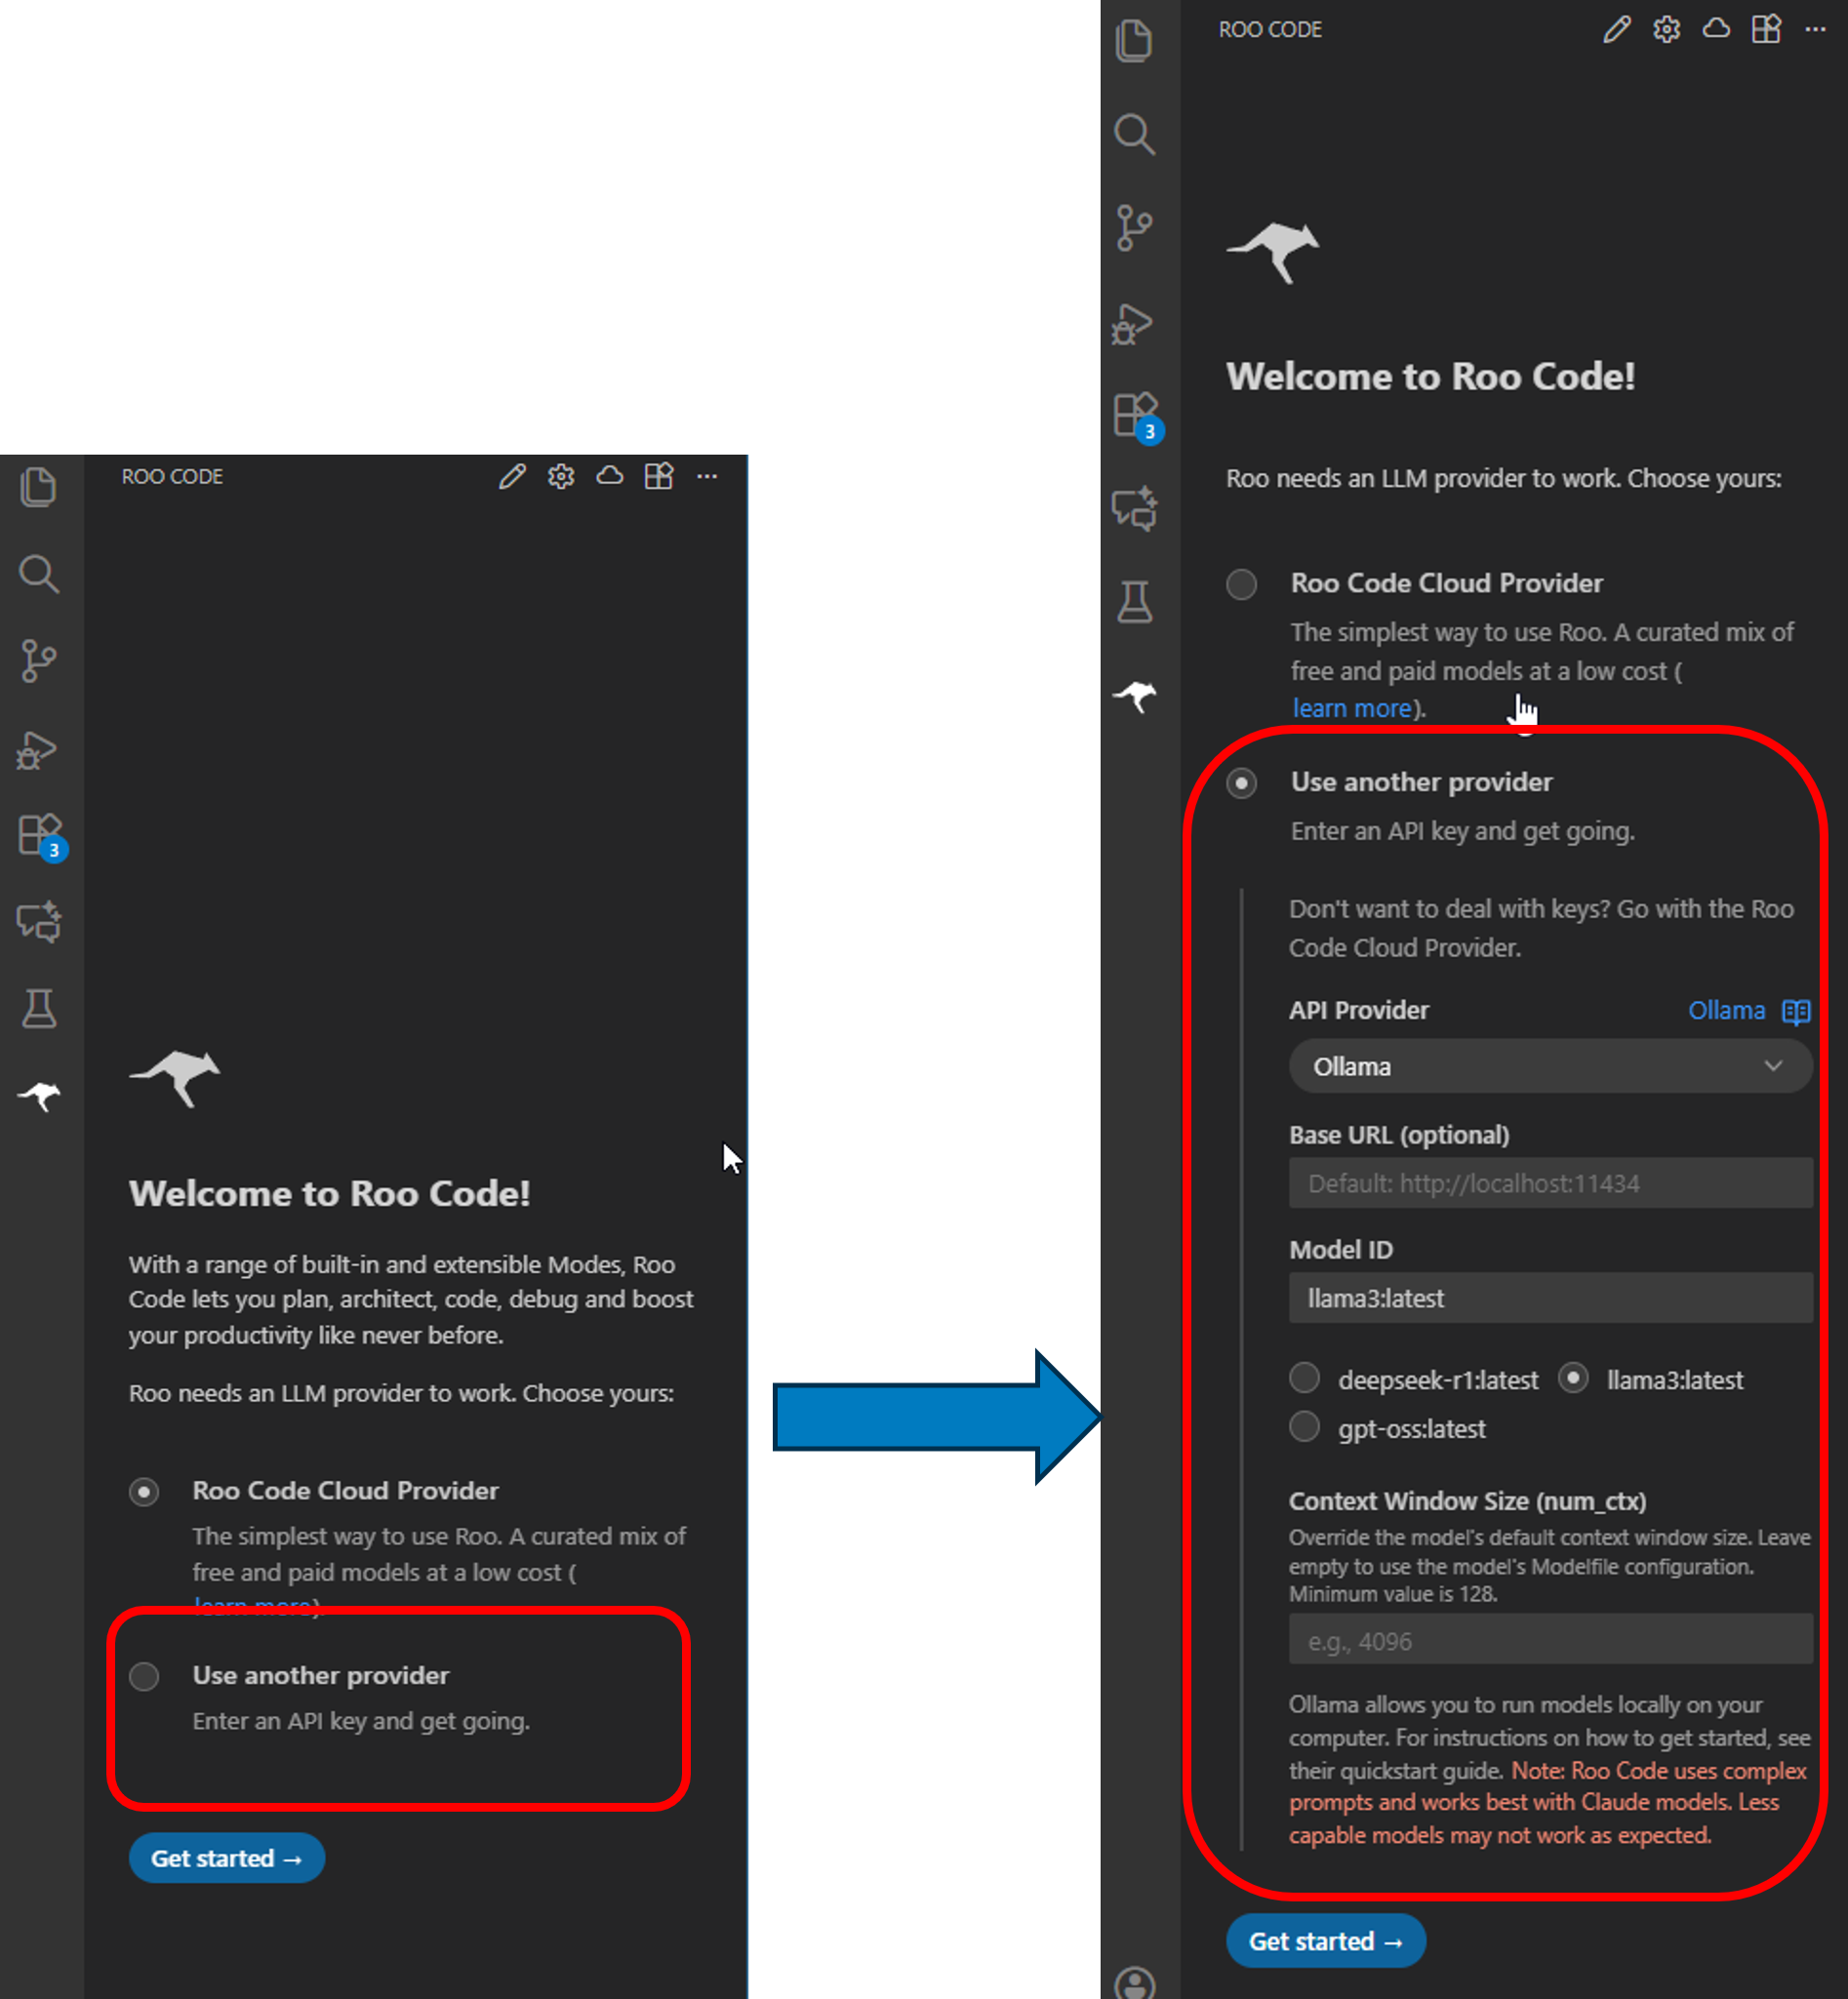
\includegraphics{./include/graphics/roocode/RooCodeUseLLMProviders.png}

\subsection{API Provider Configuration}
\begin{boxhint}{Pre-condition}
You must obtain an API Key from a provider.
List of supported AI service providers:
\begin{itemize}
   \item OpenAI
   \item Google Gemini
   \item Anthropic
   \item \dots
\end{itemize}
\end{boxhint}

\begin{enumerate}
   \item Open \textbf{VSCodium For RobotFramework}.
   \item Click the \textbf{Roo Code icon} in the Activity Bar.
   \item Click the \textbf{Settings (gear icon)} at the top of
      the Roo Code panel.
   \item Select your provider (e.g., \textbf{Anthropic} for Claude 3.5 Sonnet).
   \item Enter your \textbf{API Key}.
   \item Choose the specific model (e.g., \texttt{claude-3-5-sonnet-20241022}).
   \item Click \textbf{Done}.
\end{enumerate}

Refer to the image below for an example of using \textbf{Google Gemini} as
the API provider:

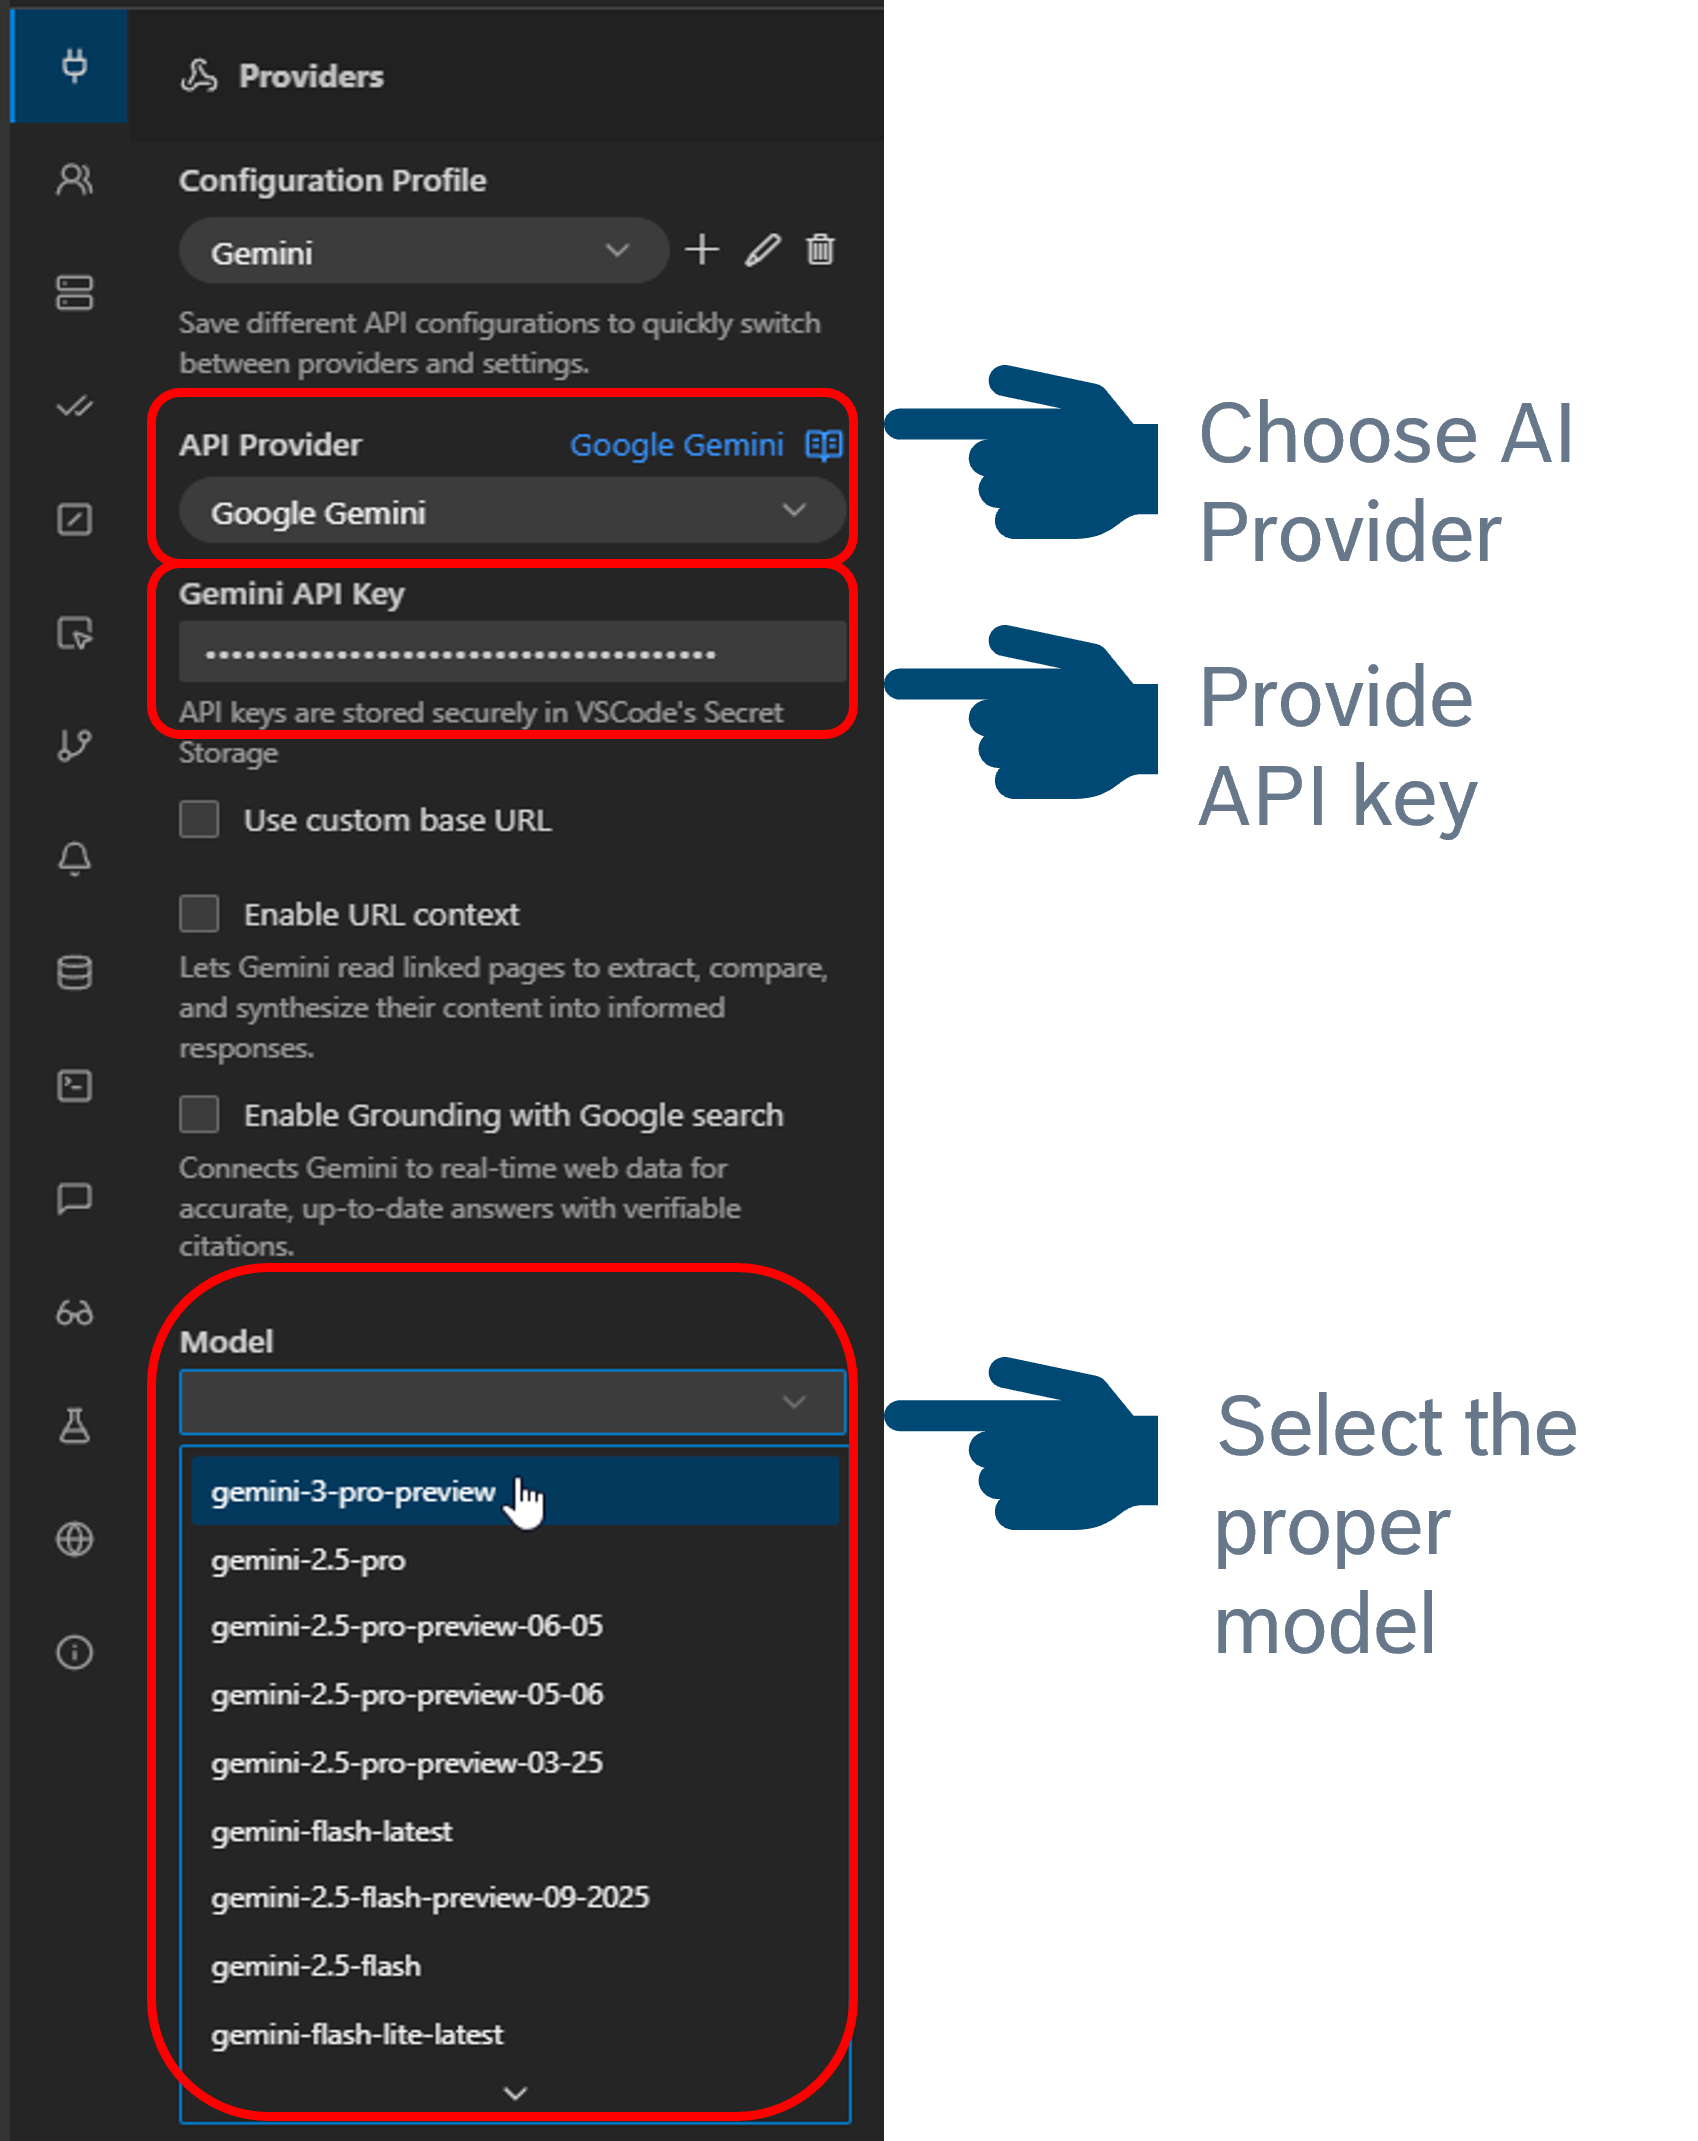
\includegraphics{./include/graphics/roocode/AIProviders.png}

\subsection{Local Model Setup (Ollama)}
For maximum privacy, you can run models locally.
\begin{boxhint}{System Requirement}
Running local models requires significant RAM/GPU resources.
\end{boxhint}

\begin{boxhint}{Pre-condition}
   You need to have Ollama installed and a local model downloaded.
   \begin{itemize}
      \item Download and install Ollama from
         \href{https://ollama.com/download}{Download Ollama}
      \item Use Ollama CLI to pull a coding model:
         \texttt{ollama pull deepseek-v3.1} or \texttt{ollama pull qwen3-coder}.
         You can find other models provided by Ollama at
         \href{https://ollama.com/library}{Ollama Library}.
      \item Ensure Ollama and pulled models are running locally on your machine.

            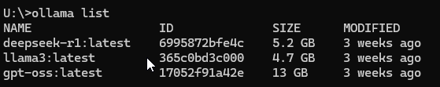
\includegraphics{./include/graphics/roocode/OllamaModels.png}
   \end{itemize}

\end{boxhint}

Steps to configure Roo Code with \textbf{Ollama}:
\begin{enumerate}
   \item Open \textbf{VSCodium For RobotFramework}.
   \item Click the \textbf{Roo Code icon} in the Activity Bar.
   \item Click the \textbf{Settings (gear icon)} at the top of
      the Roo Code panel.
   \item In the \textbf{API Provider} option, select \textbf{Ollama}
      as the provider.
   \item Ensure the Base URL is set (usually \texttt{http://localhost:11434}).
   \item Choose the local model you pulled earlier.
   \item Click \textbf{Done}.
\end{enumerate}

Refer to the image below for guidance:

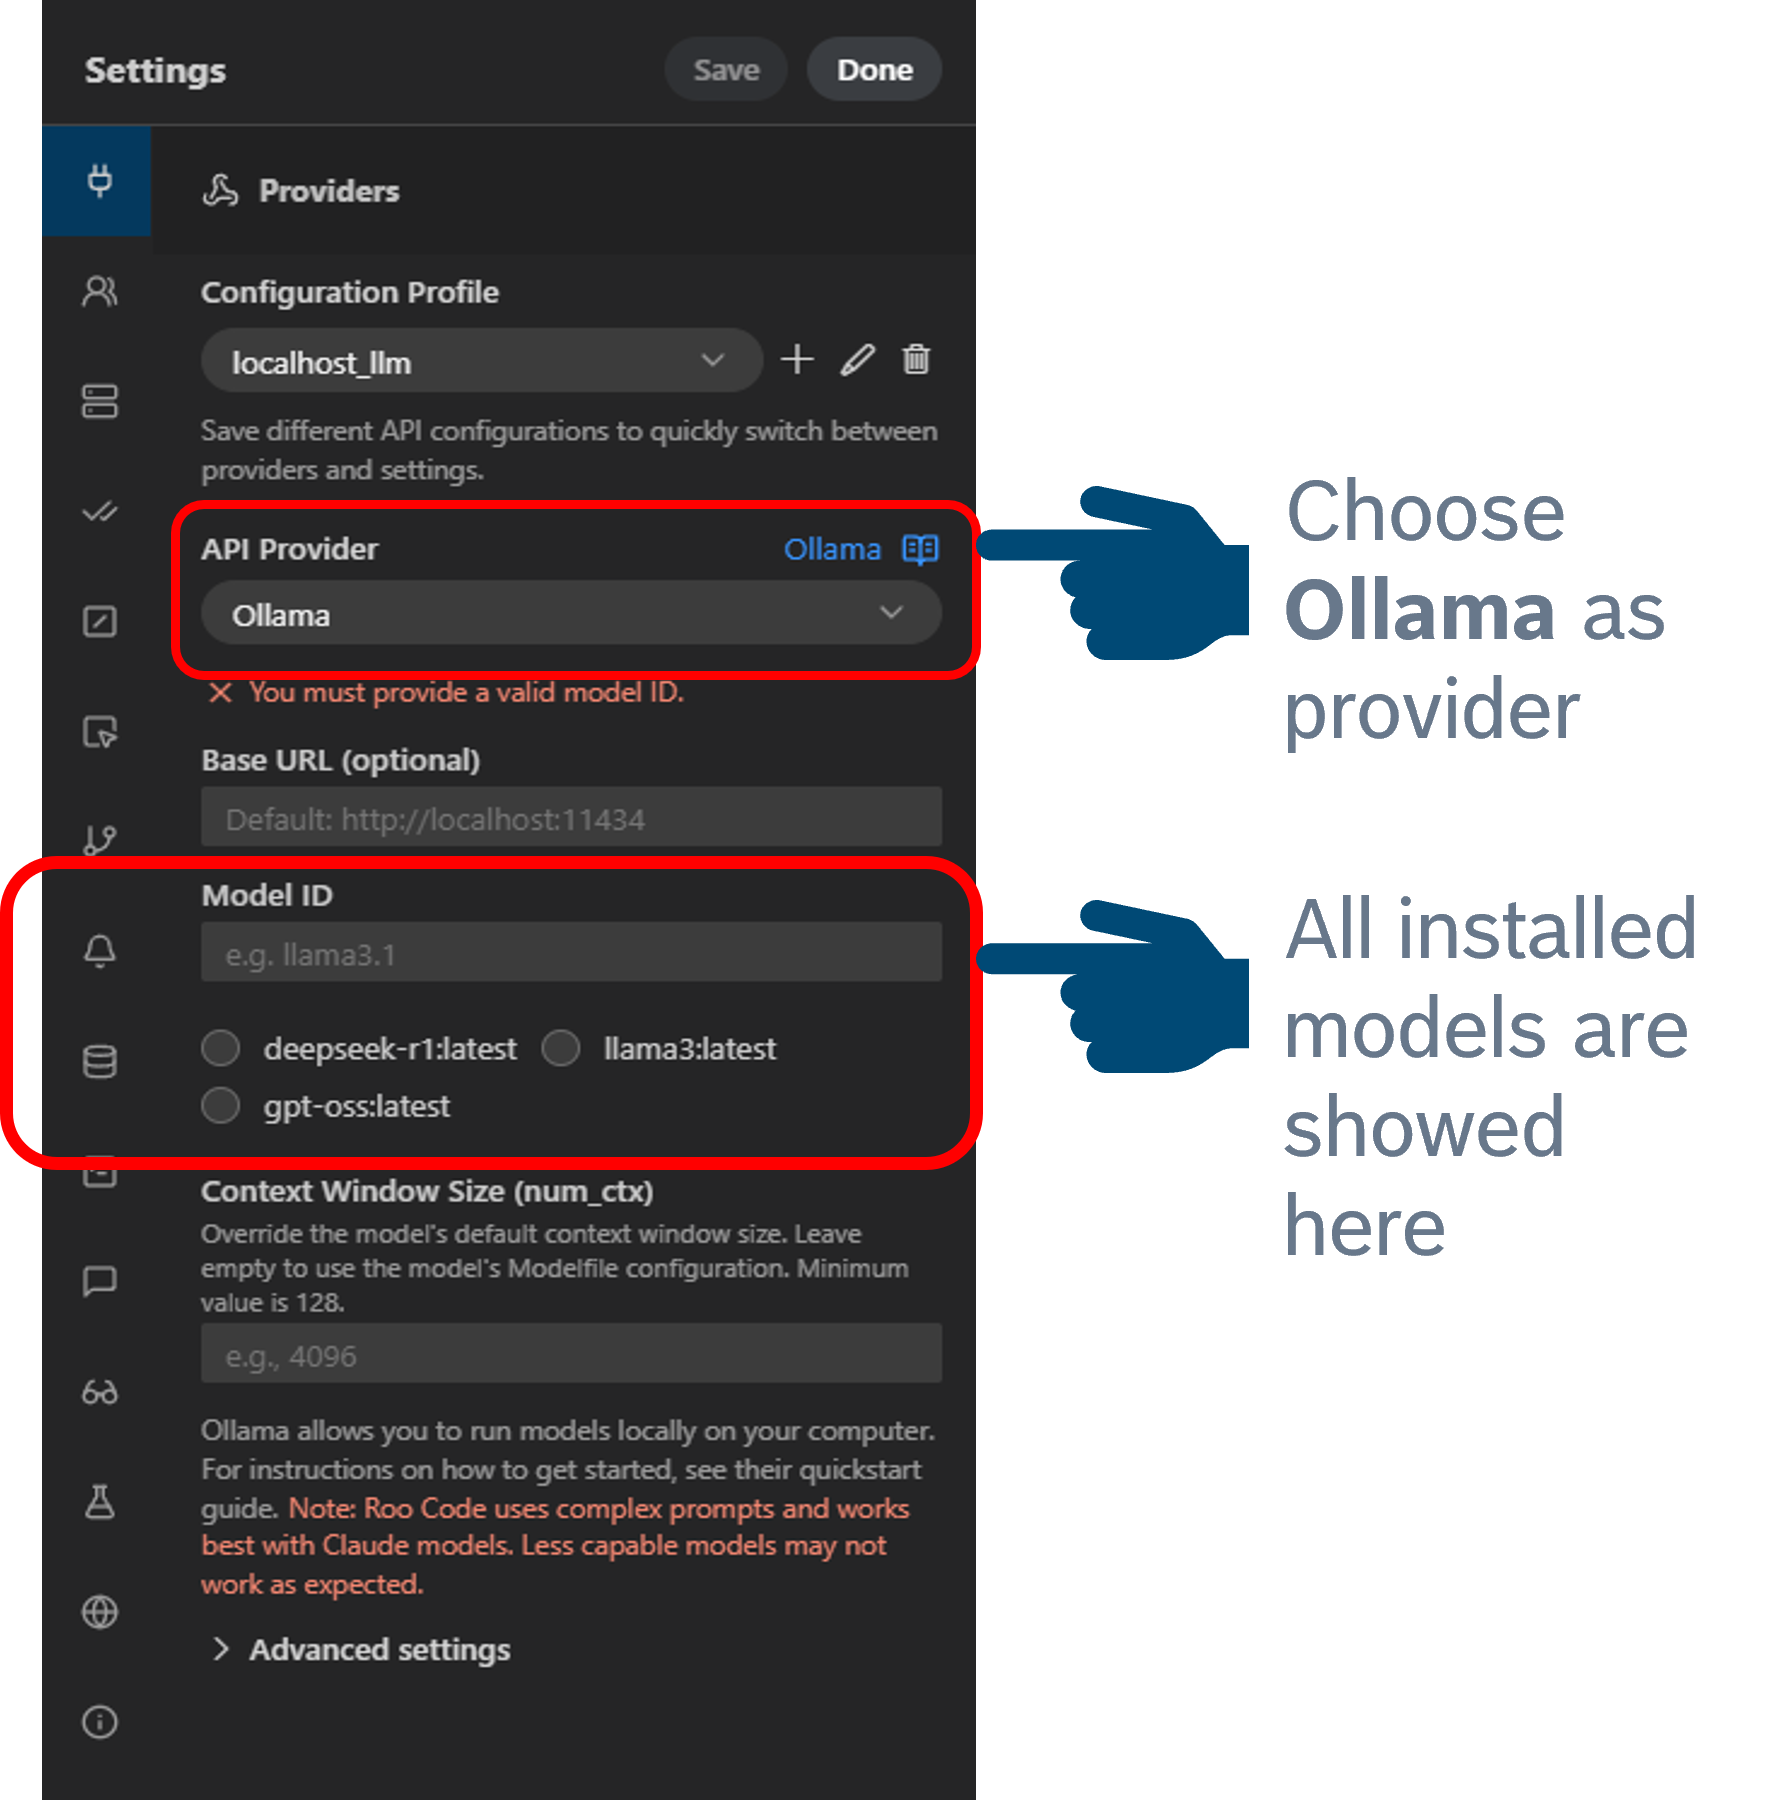
\includegraphics{./include/graphics/roocode/OllamaProvider.png}

\subsection{GitHub Copilot Integration}
Roo Code can leverage your existing GitHub Copilot subscription as
an API source.

\begin{boxhint}{Pre-condition}
Ensure the \textbf{GitHub Copilot} Extensions are installed

\includegraphics{./include/graphics/roocode/GitHubCopilotExtensions.png}
and you are signed in with your GitHub account.

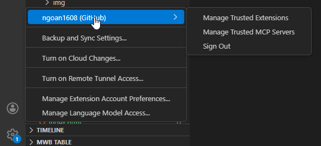
\includegraphics{./include/graphics/roocode/GithubCopilotAuth.png}
\end{boxhint}

Steps to configure Roo Code with \textbf{GitHub}:
\begin{enumerate}
   \item Open \textbf{VSCodium For RobotFramework}.
   \item Click the \textbf{Roo Code icon} in the Activity Bar.
   \item Click the \textbf{Settings (gear icon)} at the top of
      the Roo Code panel.
   \item In the \textbf{API Provider} option, select \textbf{VS Code LM API}
      as the provider.
   \item Choose the available model within the dropdown menu.
   \item Click \textbf{Done}.
\end{enumerate}

Refer to the image below for guidance:

\includegraphics{./include/graphics/roocode/GitHubCopilotLLM.png}

\section{Working Modes}
Roo Code uses specialized personas to optimize token usage and task accuracy.

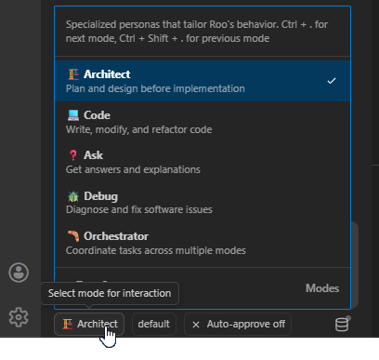
\includegraphics{./include/graphics/roocode/RooCodeModes.png}

\begin{itemize}
   \item \textbf{Architect:}
      \begin{itemize}
         \item \textbf{Goal:} Planning and high-level design.
         \item \textbf{Behavior:} Proposes solutions and analyzes code without
            making changes.
      \end{itemize}
   \item \textbf{Code:}
      \begin{itemize}
         \item \textbf{Goal:} Full implementation.
         \item \textbf{Behavior:} Has full write-access to create features,
            refactor code, and update the workspace.
      \end{itemize}
   \item \textbf{Debug:}
      \begin{itemize}
         \item \textbf{Goal:} Bug hunting and fixing.
         \item \textbf{Behavior:} Specifically designed to analyze logs,
            terminal errors, and fix broken test scripts.
      \end{itemize}
   \item \textbf{Orchestrator:}
      \begin{itemize}
         \item \textbf{Goal:} Complex task management.
         \item \textbf{Behavior:} Breaks down large objectives into smaller
            sub-tasks for execution.
      \end{itemize}
   \item \textbf{Ask:}
      \begin{itemize}
         \item \textbf{Goal:} Knowledge retrieval.
         \item \textbf{Behavior:} Acts as a read-only consultant to explain
            logic or query documentation.
      \end{itemize}
\end{itemize}

\section{Best Practices for Automation Engineers}
\begin{itemize}
   \item \textbf{Context Management:}
      Keep only relevant files open to reduce token costs.
   \item \textbf{Terminal Verification:}
      Always let Roo Code run your Robot Framework commands
      (e.g., \plog{robot path/to/test.robot}) to verify its own fixes.
   \item \textbf{Approval Workflow:}
      Carefully review the \textbf{Diff} view before clicking \textbf{"Approve"}
      to ensure the accuracy of file changes.
\end{itemize}

\section{References}
For more information and detailed documentation,
refer to the following resources:
\begin{itemize}
   \item \textbf{Roo Code Homepage:}
      \href{https://docs.roocode.com/}{docs.roocode.com}
   \item \textbf{Roo Code Tutorial Videos:}
      \href{https://docs.roocode.com/tutorial-videos}
      {https://docs.roocode.com/tutorial-videos}
   \item \textbf{Roo Code Example - First Task:}
      \href{https://docs.roocode.com/getting-started/your-first-task}
      {https://docs.roocode.com/getting-started/your-first-task}
   \item \textbf{MCP Directory:}
      \href{https://modelcontextprotocol.io/}{Model Context Protocol}
\end{itemize}
